\section{Controller}

  This chapter describes the implementation of the features elicited on the previous chapters in details, specifically within the FDS component. All the HTTP routes of the FDS will be prefixed with \verb;/api/v1;.

  \subsection{Customer Validation on a Registration Event}

    An HTTP endpoint will be implemented to provide the possibility to schedule a validation process as soon as a new customer is registered. The endpoint should accept the customer information on the request body and return validation ID and additional information of the validation process as a response. Listed below is the code snippet of the HTTP controller of the endpoint to schedule a validation process:

    \begin{lstlisting}[style=es6, caption={HTTP controller of an endpoint to schedule a validation process (TypeScript)}]
// fds/src/routes/validation/validationController.ts

// Picks the `validationId` and `additionalInfo` attributes from `Validation` 
type ValidationSchedule = Pick<Validation, "validationId" | "additionalInfo"> 
     
@Route("validate")
@Tags("Validation")
export class ValidationController extends Controller {
  @SuccessResponse(201, "Validation started")
  @Response<ValidationErrorJSON>(422, "Validation Failed")
  @Response<WentWrong>(400, "Bad Request")
  @Post()
  public async validateCustomer(
   @Body() requestBody: Customer
  ): Promise<ValidationSchedule | WentWrong> {
    const result = await ValidationService.scheduleRulesetValidation(requestBody)
    const { data, error } = result

    if (error) {
      this.setStatus(400)
      return {
        message: error.message,
        details: error.details || "",
      }
    }

    return data
  }
} 
    \end{lstlisting}
    
    The HTTP controller is intentionally kept as simple as possible. The logic behind the process to schedule a validation is done by the \verb;ValidationService; and \verb;ValidationEngine; (discussed in \autoref{sub:process}). The \verb;ValidationService; is responsible in this particular case to get the lists of existing validation rules and runtime secrets (discussed in \autoref{sub:secrets}), then creating a new instance of \verb;ValidationEngine; as well as scheduling a new validation process. 

    \begin{lstlisting}[style=es6, caption={ValidationService schedule validation implementation (TypeScript)}]
// fds/src/routes/validation/validationService.ts

export class ValidationService {
  static async scheduleRulesetValidation(
    customer: Customer
  ): Promise<ApiResponse<ValidationSchedule>> {
    const { data: ruleset, error } = await RulesService.listRules()
    const secrets = await SecretsService.listSecrets()
    if (error) {
      return {
        data: null,
        error,
      }
    }

    const { validationId, additionalInfo } = await new ValidationEngine<Customer>()
      .setRuleset(ruleset)
      .setSecrets(secrets)
      .scheduleRulesetValidation(customer)

    return {
      data: {
        validationId,
        additionalInfo,
      },
      error: null,
    }
  }
}
    \end{lstlisting}

  \subsection{Validation Process}
    \label{sub:process}

    \subsubsection{Validation Process Flow}
    
      A validation process is started by iterating through a list of validation rules, making an HTTP request to the external endpoint listed on each rule and evaluating its response in comparison to the conditions attached on the rule. If the HTTP response from the external matches the conditions of the rule, the rule evaluation will be considered as a passed evaluation, otherwise it is a failed evaluation. The result of each rule evaluation determines the value of the resulting fraud score. The resulting fraud score will be calculated as follows: 

      \begin{itemize}
        \item Initialize an empty list of fraud scores. The list will be filled later with float numbers ranging between 0 and 1
        \item Go through the list of validation rules and run evaluation
        \item If the evaluation passed, append \verb;0; to the list of fraud scores
        \item Otherwise, append the validation rule \verb;failScore; attribute's value to the list of fraud scores
        \item At the end of the iteration, the list size should equal to the amount of available\footnote{\emph{Not skipped.}} validation rules
        \item The resulting fraud score is the sum of the scores in the list, divided by the number of available validation rules
      \end{itemize}
      
      In summary, the flow of a validation process will be represented by the flow diagram below:

      \begin{figure}[!ht]
        \centering
        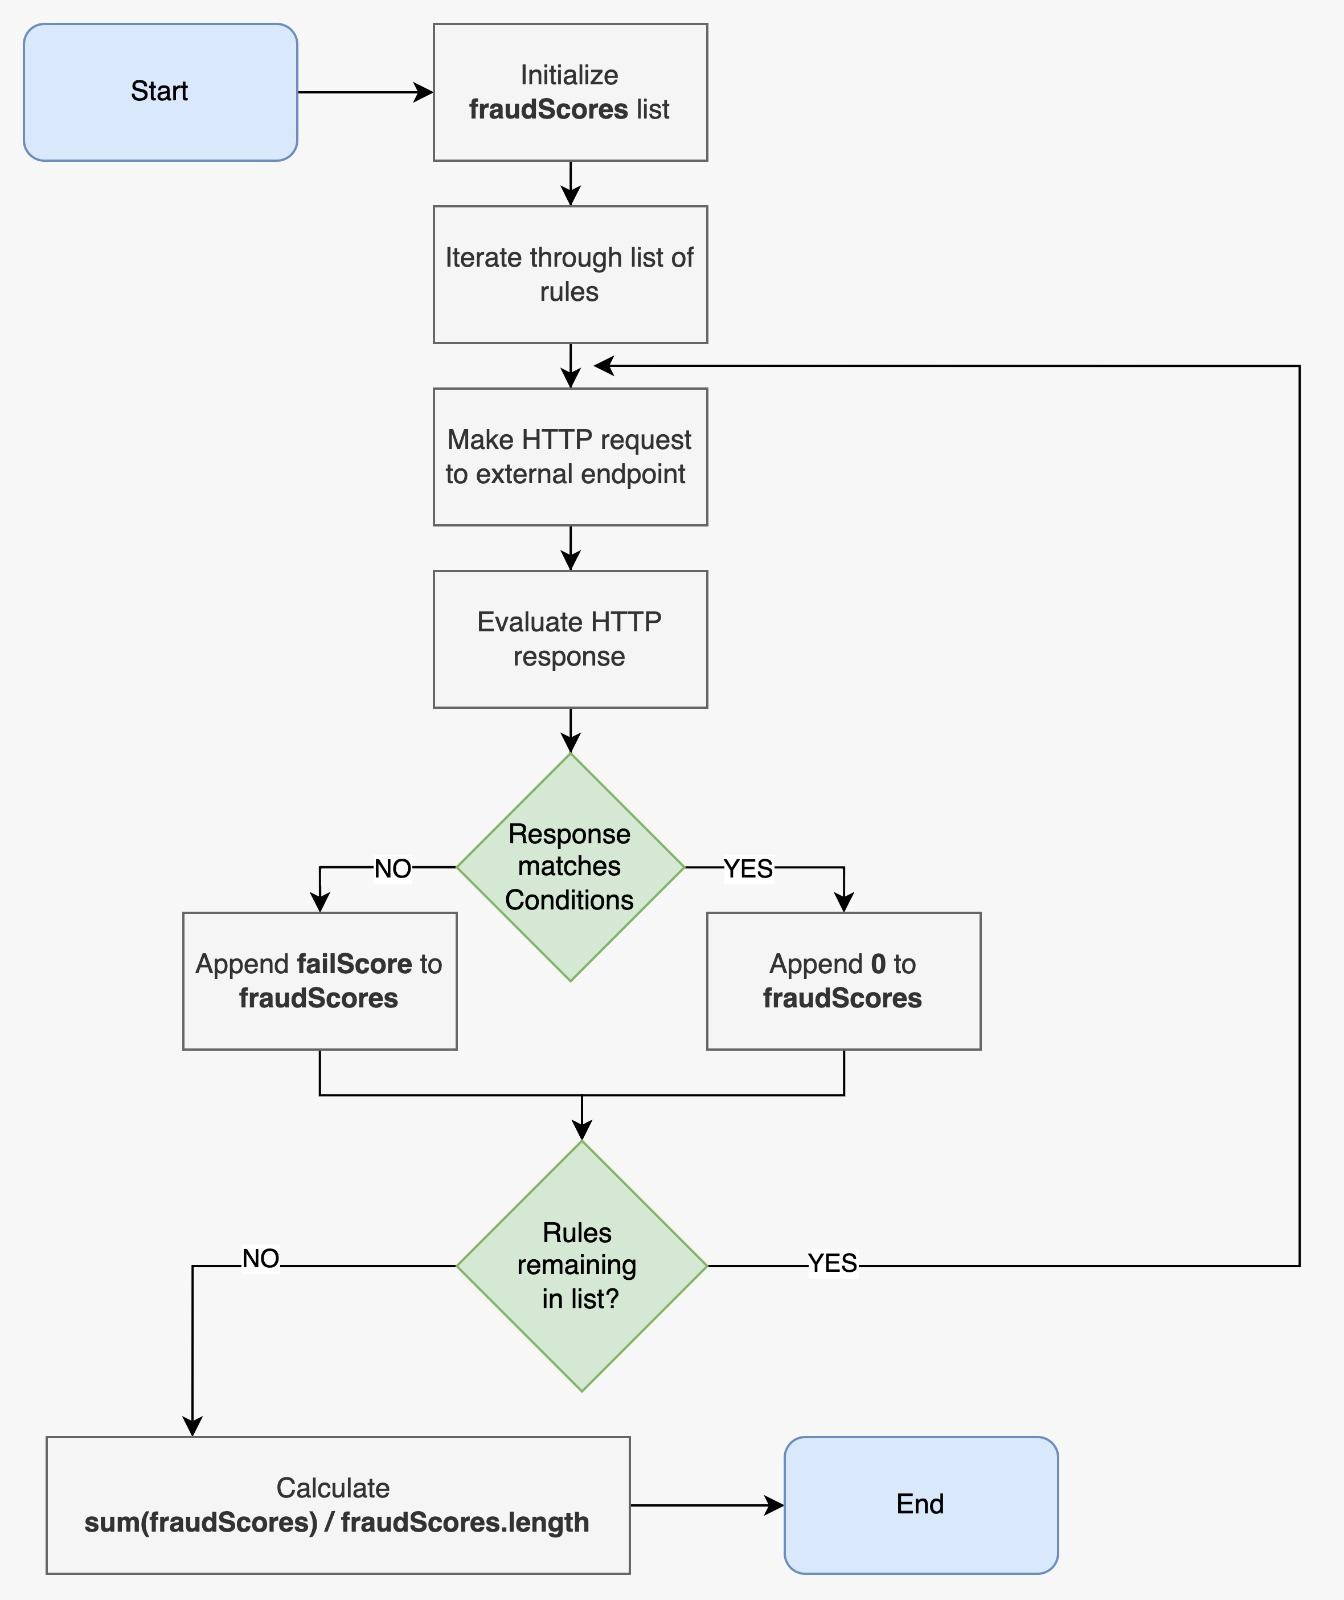
\includegraphics[width=0.8\textwidth]{diagrams/flow_validation_process.jpeg}
        \caption{Flow diagram of a validation process}
        \label{fig:flow_validation}
      \end{figure}
      
      The flow listed above will be executed by creating a \verb;ValidationEngine; instance and calling a public \verb;secheduleRulesetValidation; method. Before running a validation process, the list of validation rules as well as runtime secrets should be provided to the engine. The \verb;ValidationEngine; class uses method chaining\footnote{\emph{Method chaining} is a method to provide the possibility of invoking multiple method calls of an object without having to store an intermediary result in an additional variable.} as well as the \emph{Builder} design pattern discussed in \autocite[pp. 97-106]{gamma-1995} for its construction, to make the public API of a validation engine as simple as possible.

      \begin{lstlisting}[style=es6, caption={ValidationEngine class and the scheduleRulesetValidation method (TypeScript)}]
// fds/src/engine/valdiationEngine.ts
export class ValidationEngine<T> {
  private secrets: GenericObject = {}
  private ruleset: ValidationRule[] = []

  setSecrets(secrets: GenericObject) {
    this.secrets = secrets
    return this
  }

  setRuleset(ruleset: ValidationRule[]) {
    this.ruleset = [...ruleset.sort((a, b) => b.priority - a.priority)]
    return this
  }

  async scheduleRulesetValidation(data: T): Promise<Validation<T>> {
    if (this.ruleset.length === 0) {
      throw new Error("Ruleset is not set")
    }

    await this.constructValidationObject(data) // Construct a validation result
    this.validateRuleset(data)

    return this.validationResult
  }

  async validateRuleset(data: T): Promise<Validation<T>> {
    if (this.ruleset.length === 0) {
      throw new Error("Ruleset is not set")
    }

    if (!this.validation) {
      await this.constructValidationObject(data)
    }

    for await (const rule of this.ruleset.filter(({ skip }) => !skip)) {
      const evaluationResult = await this.evaluateRule(rule, data)
      await this.reviewEvaluationResult(evaluationResult, rule)
    }

    await this.afterValidation()

    return this.validationResult
  }
}
      \end{lstlisting}

    \subsubsection{Making an HTTP Request to External Endpoints}

      A dedicated class (\verb;Agent;) is created to make an HTTP request to the external endpoint. The class will provide a layer of abstraction on top of the Got library that is being used to actually make the HTTP requests. 
      
      The class will also help in setting the request body, request header as well as to change the variables on the \verb;endpoint; attribute with its corresponding values. The class follows the \emph{Singleton} design pattern described in \autocite[pp. 127-134]{gamma-1995}, as there might only one instance needed for the whole application. The class is also implemented using the dependency injection in mind, for an easier access to the underlying library during the testing phase. 

      \begin{lstlisting}[style=es6, caption={Agent class, to make HTTP requests to the external endpoints (TypeScript)}]
// src/fds/engine/request/agent.ts
export class Agent {
  private static context: Context // Dependency injection

  private static get client() {
    return Agent.context.client
  }

  static setClient(context: Context) {
    this.context = context
  }

  static async fireRequest<DataType, ResponseType = string>(
    rule: ValidationRule,
    data: DataType,
  ): Promise<FireRequestReturnType> {
    const { method, retryStrategy } = rule

    try {
      const response = await this.client<ResponseType>(this.getUrl(rule, data), {
        method: method as Method,
        retry: retryStrategy || {},
        headers: this.getHeader(rule, data),
        json: this.getJSONBody(rule, data),
      })

      const { statusCode, statusMessage, body, rawBody, retryCount } = response

      return {
        error: null,
        data: {
          statusCode,
          statusMessage,
          rawBody,
          retryCount,
          body: this.parseResponseBody(body),
        },
      }
    } catch (e) {
      return {
        error: {
          message: e,
        },
        data: null,
      }
    }
  }
}
      \end{lstlisting}

      The attributes returned by the request agent is specifically chosen, as returning the whole response object might not be beneficial. 
      
      As there might be dynamic values listed on the \verb;requestBody, requestHeader; or \verb;requestUrlParameter; attributes of a validation rule\footnote{A dynamic value is marked by providing a JSONPath expression as the value in the key-value pairs of the corresponding attribute.}, a helper function to query the associated attribute by evaluating the JSONPath expression provided is implemented within the \verb;Agent; class. 

      \begin{lstlisting}[style=es6, caption={Accessing data on runtime (TypeScript)}]
// fds/src/engine/request/agent.ts
import jp from "jsonpath"

export class ValidationEngine<T> {
  private static accessDataFromPath([key, value]: [string, any], data: any) {
    if (typeof value !== "string") {
      return {
        [key]: value,
      }
    }

    const SEPARATOR = " "
    const splitted = value.split(SEPARATOR)
    return {
      [key]: splitted
        .map((chunk) => {
          try {
            const dataFromPath = jp.query(data, chunk)[0]
            return dataFromPath ?? chunk
          } catch {
            return chunk
          }
        })
        .join(SEPARATOR),
    }
  }
}
      \end{lstlisting}

    \subsubsection{Evaluating a Rule} 

      \begin{lstlisting}[style=es6, caption={Rule evaluation in ValidationEngine (TypeScript)}]
// fds/src/engine/validationEngine.ts
export class ValidationEngine<T> {
  private async evaluateRule(
    rule: ValidationRule,
    data: T,
  ): Promise<EvaluationResult> {
    const { endpoint, retryStrategy, condition, name } = rule

    const validationEvent = this.validation.events.find(
      (event) => event.name === name,
    )
    
    if (validationEvent) {
      validationEvent.dateStarted = new Date().toISOString()
      validationEvent.status = "RUNNING"
      await this.pushToDatastore()
    }

    const { error, data: responseData } =
      await Agent.fireRequest(rule, {
        customer: data,
        secrets: this.secrets,
      })

    if (error) {
      return {
        messages: [
          `${(*@\textcolor{black}{endpoint}@*)} is not accessible.${
            (*@\textcolor{black}{retryStrategy}@*)
              ? ` (*@\textcolor{forestgreen}{Retries done:}@*) ${retryStrategy.limit}`
              : ""
          }`,
          error.message,
        ],
        pass: false,
      }
    }

    const evaluator = EvaluatorFactory.getEvaluator(condition)
    return evaluator.evaluate({
      response: responseData,
      customer: data,
      secrets: this.secrets,
    })
  }
}
      \end{lstlisting}
      
      

  \subsection{Notification on Suspicious Cases}

  \subsection{Validation Rules Management}

  \subsection{Validation Real Time Progress}

  \subsection{Runtime Secrets}
    \label{sub:secrets} 

  \subsection{Error Handling}

